% Chapter 4

\chapter{Progettazione} % Main chapter title

\label{Chapter4} % Change X to a consecutive number; for referencing this chapter elsewhere, use \ref{ChapterX}

Così come nella progettazione di un software si passa dall'analisi alla sua progettazione, prima di svilupparlo. Anche in questo caso, è opportuno progettare l'intero cortometraggio, prima di realizzarlo.
Questo è un passaggio importante poiché non solo permette di capire come il prodotto dovrà essere realizzato, ma permette anche di stabilire delle convenzioni standard (e.g. nomi dei file) da mantenere durante il progetto.
Quest'ultimo aspetto è indispensabile soprattutto nel caso in cui ci siano più persone a lavorare allo stesso progetto.

%----------------------------------------------------------------------------------------
%	SECTIONS
%----------------------------------------------------------------------------------------

\section{Progettazione generale}

%finish your film "Design"
Normalmente la fase di progettazione di un cortometraggio serve a definire l'aspetto dei personaggi e dell'ambientazione (i.e. Character Design, Environment/Prop Design).
Tuttavia questi aspetti sono stati prevalentemente coperti da A. Uras, in quanto il corto rappresenta una storia di sua creazione, e non verranno trattati. La progettazione delle animazioni verrà invece trattata dettagliatamente, in quanto oggetto principale del mio lavoro.

A questo punto del progetto era chiaro che l'obiettivo finale era quello di realizzare un breve trailer di una possibile serie piuttosto che un cortometraggio.
Si è quindi proceduti a selezionare le scene da realizzare per stare entro i due minuti di tempo di riproduzione.

Fatto ciò ho proceduto col creare un flusso di lavoro, in maniera tale da procedere in modo organizzato.
Siccome non ero il solo a lavorare a questo progetto ho scelto un approccio orientato alla produzione, ovvero in cui diversi team si occupano di diversi aspetti del progetto ma che, ciò non di meno, sono collegati e dipendono gli uni dagli altri.

Ad esempio, una volta realizzato il rig base per un modello dev'essere possibile animarlo direttamente, anche senza avere il rig avanzato finale. Ancora più importante è che sia possibile aggiungere dettagli ad un modello, come materiali e textures, anche dopo che questo è stato animato.
Per fare ciò, ho seguito una semplice filosofia: creare l'oggetto una volta e linkarlo in diverse scene invece che copiarlo.
Questa procedura è analoga a quella di utilizzare delle interfacce nella programmazione ad oggetti invece che le classi direttamente. In questo modo, è possibile modificare una classe in un secondo tempo senza alterarne il suo comportamento e, di conseguenza, chi la utilizza non nota alcuna differenza.

Ciò è stato possibile anche grazie alla caratteristica delle armature (o scheletro), di poter essere animate anche quando linkate da un altro file.
In pratica, è possibile definire un proxy che permette di accedere a tutte le proprietà di un'armatura come se questa fosse l'oggetto originale e non una copia (o meglio un link).

\section{Progettazione delle animazioni}

Quando si tratta di sviluppare qualcosa di complesso come una figura umana, è opportuno progettarla, per trovare un modello di astrazione che la semplifichi, pur mantenendo le proprietà che ci interessano e quindi ci permetta di animarla in maniera efficiente.
Il corpo umano è infatti composto da circa duecento DOF \cite{Parent:2012:CAA:2385444}.
Nonostante ciò, la struttura esteriore è fondamentalmente composta da un'unica mesh.
Quindi, rispetto a quanto visto fin'ora, dove la struttura da animare era un'armatura composta da più ossa, sarà necessario deformare la mesh per adattarla all'armatura sottostante. Ciò è possibile associando determinati vertici della mesh ad ogni osso.

La progettazione del rig (Figura \ref{fig:rig}) serve ad ottenere una serie di controlli interattivi mirati a facilitare l'animazione del personaggio.
L'usabilità di un rig è un aspetto fondamentale, in quanto, se il rig non è semplice da utilizzare per un animatore, esso è completamente inutile.
Il rig, infatti, non è fine a se stesso, ma è lo strumento che permettera (solitamente ad altri) di animare i nostri modelli.
La progettazione delle animazione consiste dunque nell'ideare un rig che ci permetterà poi di animare i medelli efficientemente. Parlare di progettazione di animazioni o di rig è quindi indifferente.
Per progettare un buon rig serve, prima di tutto, individuarne l'obiettivo, per rendere il rig il più semplice possibile.
Di seguito sono riportati alcuni degli obiettivi individuati e per le dverse parti di un rig.

\newpage
\subsection{Arti superiori}

\begin{figure}
\centering
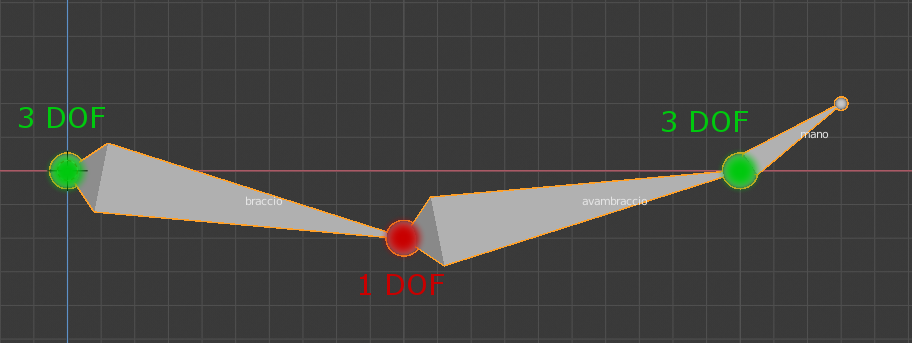
\includegraphics[width=.8\textwidth]{Figures/arm}
\decoRule
\caption[Rig braccio]{Esempio di un semplice rig per il braccio.}
\label{fig:arm}
\end{figure}

Le braccia devono essere in grado di estendersi per raggiungere e afferrare oggetti.
Come spiegato in precedenza (Capitolo \ref{Chapter3}), ha senso fare utilizzo dell'IK per posizionare la mano dove si vuole, e lasciare che il resto del braccio venga posizionato di conseguenza.
In tal caso è opportuno identificare quante articolazioni sono necessarie nel braccio e quanti DOF servono in ciascuna di esse.
Un buon modo di rappresentare gli arti superiori è quello di utilizzare 7 DOF: 3 per la spalla e il polso, 1 per il gomito (vedi Figura \ref{fig:arm}).

Un altro modo è quello di aggiungere un articolazione a metà dell'avambraccio per permettere la rotazione longitudinale di esso.
In altri casi l'avambraccio è staccato dal braccio, questo permette di evitare di dover deformare la mesh, ma il taglio netto tra avambraccio e braccio non sempre è conveniente in termini di visualizzazione.
Per tutte le figure umane nel nostro progetto è stata utilizzata la prima rappresentazione (Figura \ref{fig:arm}).
Nel corto, appaiono anche dei robot, per i quali sarebbe potuto essere utilizzata la terza rappresentazione, più semplice.
È stato tuttavia scelto di utilizzare comunque la prima per permettere di avere lo stesso scheletro per tutti i personaggi, in modo da avere un rig uniforme e non dover fare del lavoro doppio.

Un'ultima considerazione da fare è che ci sono alcuni casi in cui è preferibile poter animare il braccio attraverso FK.
Per questo motivo è stato scelto di utilizzare un rig che permetta di alternare tra FK e IK.
Nel caso della FK è inoltre opportuno rendere la rotazione del braccio indipendente da quella del corpo.
Questa caratteristica è quasi sempre indispensabile, se si pensa ad esempio al ritardo del movimento delle braccia, quando quando le si lascia andare (a peso morto), rispetto a quello del busto, facendolo ruotare a destra e sinistra.
Esistono  però dei casi in cui è preferibile che le braccia mantengano la rotazione del busto, ad esempio nel caso di un robot.
Siccome lo stesso rig verrà utilizzato sia per umani che robot, ha senso far si che questa caratteristica sia attivabile e disattivabile a seconda di chi stia implementando il rig.

\begin{figure}
\centering
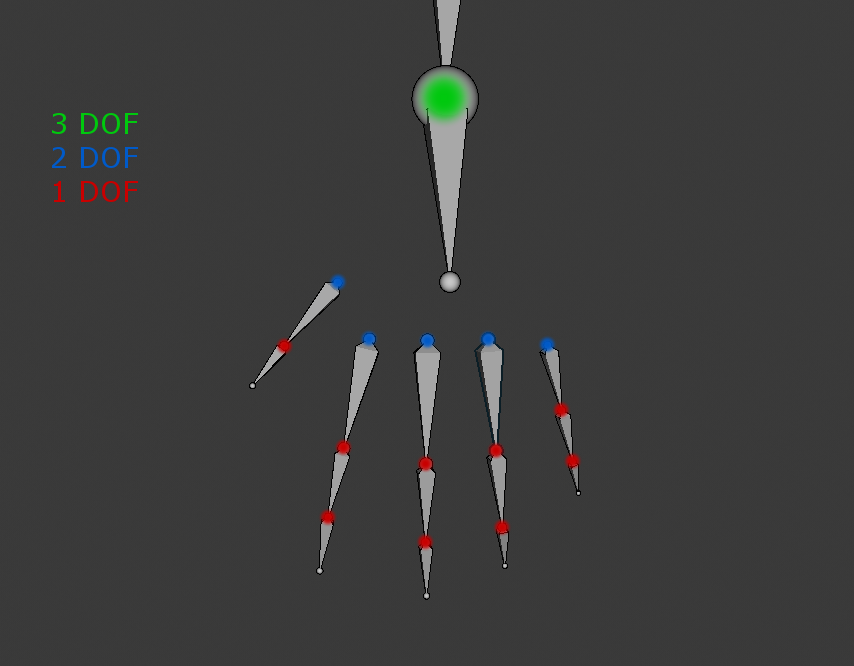
\includegraphics[width=.8\textwidth]{Figures/hand}
\decoRule
\caption[Rig mano]{Esempio di un semplice rig per la mano}
\label{fig:hand}
\end{figure}

\newpage
Per quanto riguarda il rig della mano un modello molto utilizzato è quello rappresentato in Figura \ref{fig:hand}.
In alcuni casi un osso aggiuntivo è presente per ogni dito, tra la falange e il polso, per permettere un maggiore controllo e livello di dettaglio.
Nel nostro caso, questa scelta non è stata ritenuta necessaria, preferendo un rig più semplice e più veloce da animare. 
Un modo più semplice invece, soprattutto usato in videogiochi che utilizzano il minor numero possibile di poligoni, è quello di raggruppare alcune dita.
È molto importante scegliere il giusto bilancio tra livello di controllo e semplicità d'uso, questo trade-off infatti non permette di massimizzare entrambe le caratteristiche.
Siccome per le dita non è necessario avere un IK, non sono necessarie ulteriori progettazioni. Verrà semplicemente usato l'FK per il resto della mano.

Ora che le articolazioni sono state individuate e, per ciascuna di esse, si sa quanti DOF serviranno, è possibile procedere con la scelta della giusta rappresentazione di rotazione (\ref{Section3.1} Rappresentazioni di rotazione).
Basandoci su quanto visto nel Capitolo \ref{Chapter3}, si può dedurre che per le articolazioni con 3 DOF andranno utilizzati dei quaternioni. Mentre per le altre è possibile usare gli angoli di Eulero.

Nel caso di rotazione euleriana è anche necessario scegliere l'ordine degli assi, in base a quelli sui quali verrà effettuata la rotazione:
\begin{itemize}
    \item più usato -> anello (Figura \ref{fig:euler}) esterno, allineato globalmente/osso genitore;
    \item secondo più usato -> anello interno, rotazione locale;
    \item meno usato/non usato -> secondo, causa gimbal lock;
\end{itemize}

\subsection{Arti inferiori}

\begin{figure}
\centering
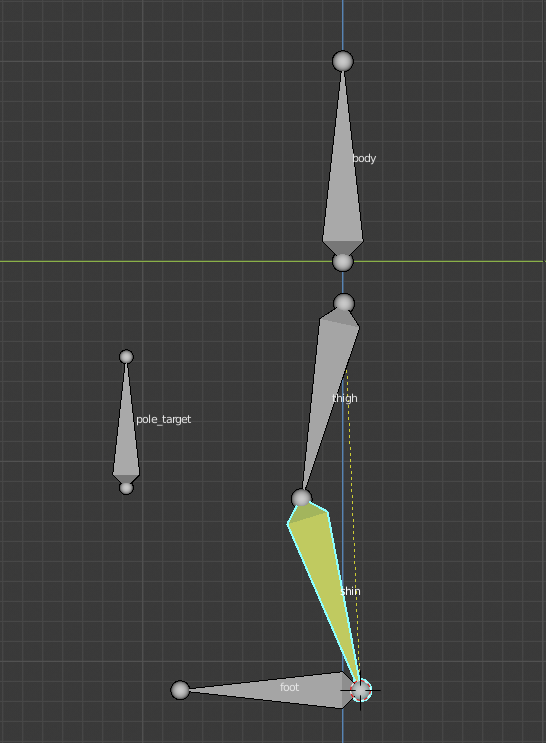
\includegraphics[width=.8\textwidth]{Figures/leg}
\decoRule
\caption[Rig gamba]{Esempio di un semplice rig per la gamba}
\label{fig:leg}
\end{figure}

Per progettare il rig delle gambe in maniera che sia efficacie, bisogna pensare a qual è il modo più conveniente di animare una camminata.

Ad un certo punto il piede poggia a terra e deve rimanere fisso in quella posizione. Il corpo, invece, continua a spostarsi in avanti.
Se usassimo la cinematica diretta, ogni volta che il corpo viene spostato in avanti, dovremmo riposizionare il piede nella posizione in cui era (i.e. counter-animation), in quanto quest'ultimo è discendente del corpo.
In alternativa potremmo rimodellare l'intera gerarchia per far si che il piede si trovi più in alto nella gerarchia rispetto al corpo. Ma questo sarebbe una pessima scelta per ovvi motivi.
Come nell'esempio della mano sulla maniglia, anche qui serve utilizzare una IK, per muovere il resto del corpo indipendentemente dal piede.
Le gambe possono quindi essere controllate interamente attraverso la cinematica inversa (Sezione \ref{sectionIK}).
Siccome questo metodo è sotto-vincolato (i.e. esistono più soluzioni), resta da specificare un vincolo aggiuntivo, relativo all'articolazione intermedia (il ginocchio).

Per fare ciò, è possibile aggiungere un osso, figlio del piede, che servirà per direzionare il ginocchio.
Il motivo per cui, quest'ultimo osso, viene solitamente definito come figlio del piede, è per il semplice motivo che piede e ginocchio puntano solitamente nella stessa direzione.
In questo modo il ginocchio eredita la rotazione del piede, semplificando ulteriormente il lavoro dell'animatore.

In blender questo osso viene chiamato \emph{Pole Target} \cite{blendDoc}, ed il suo funzionamento è molto semplice: tracciando una linea immaginaria dalla base della gamba all'end-effector, viene individuato l'asse che collega i due poli della sequenza delle ossa che costituisce la cinematica inversa.
In Figura \ref{fig:leg} questo asse è rappresentato da una linea tratteggiata gialla.
Ruotando l'intera sequenza di ossa intorno a questo asse, si ottengono infinite soluzioni ammissibili, in cui l'articolazione del ginocchio è l'unica a cambiare posizione, descrivendo una sorta di "equatore" intorno all'asse.
Ora, tracciando un'altra linea, che collega la base del \emph{pole target} all'asse precedentemente menzionato, e perpendicolare a quest'ultimo, avremo un modo di rappresentare la posizione esatta del ginocchio, attraverso l'angolo formato da quest'ultima linea rispetto alla posizione originale.
Si noti che la seconda linea rimane sempre perpendicolare all'asse. Quindi una traslazione del \emph{pole target} parallela all'asse, non ha effetto sulla rotazione della gamba.

In fine, come è stato fatto per il gomito, si può forzare il ginocchio a piegarsi su un singolo asse, garantendo un movimento ancora più realistico in fase di animazione.


